\documentclass[aspectratio=169]{beamer}
\usetheme{metropolis}
\usecolortheme{crane}

\usepackage{amsmath, amssymb}
\usepackage{tikz}
\usepackage{xcolor}
\usepackage{fontawesome5}

\usetikzlibrary{trees, positioning, arrows.meta}

% Custom colors for red-black trees
\definecolor{rbred}{RGB}{220, 38, 127}
\definecolor{rbblack}{RGB}{33, 33, 33}
\definecolor{rbgray}{RGB}{200, 200, 200}

% TikZ styles for tree nodes
\tikzset{
    rbnode/.style={circle, draw, thick, minimum size=8mm, font=\small\bfseries},
    rednode/.style={rbnode, fill=rbred!20, text=rbred, draw=rbred},
    blacknode/.style={rbnode, fill=rbblack!10, text=rbblack, draw=rbblack},
    nilnode/.style={rbnode, fill=rbgray!30, text=rbgray, draw=rbgray, minimum size=6mm}
}

\title{Red-Black Trees}
\subtitle{Why Even the Inventor Moved On...}
\author{Your Name}
\date{\today}

\begin{document}

% Title Slide
\begin{frame}
    \titlepage
\end{frame}

% Introduction - We all love to sort things
\begin{frame}{We All Love to Sort Things!}
    \begin{columns}
        \column{0.5\textwidth}
        \begin{itemize}
            \item<1-> Organizing bookshelves
            \item<2-> Arranging files on computers  
            \item<3-> Putting groceries in order
            \item<4-> \textbf{What's a really good way?} \faIcon{tree}
        \end{itemize}
        
        \column{0.5\textwidth}
        \only<4->{
            \begin{center}
                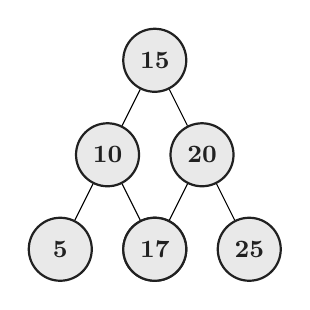
\begin{tikzpicture}[scale=0.8]
                    \node[blacknode] {15}
                        child {node[blacknode] {10}
                            child {node[blacknode] {5}}
                            child {node[blacknode] {12}}
                        }
                        child {node[blacknode] {20}
                            child {node[blacknode] {17}}
                            child {node[blacknode] {25}}
                        };
                \end{tikzpicture}
            \end{center}
        }
    \end{columns}
    
    \vspace{0.5cm}
    \only<5->{\begin{center}\Large\textbf{Binary Trees are Awesome!}\end{center}}
\end{frame}

% Why binary trees are good
\begin{frame}{Why Binary Trees Are Good}
    \begin{columns}
        \column{0.6\textwidth}
        \begin{block}{Beautiful Structure}
            \begin{itemize}
                \item Everything has its place
                \item Search: $O(\log n)$ 
                \item Insert: $O(\log n)$
                \item Delete: $O(\log n)$
            \end{itemize}
        \end{block}
        
        \pause
        
        \begin{alertblock}{The Magic}
            Logarithmic time = \textbf{Sports car performance!}
        \end{alertblock}
        
        \column{0.4\textwidth}
        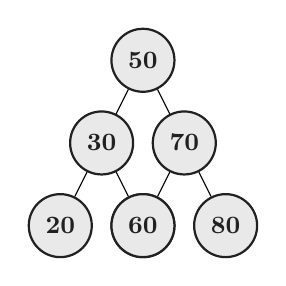
\begin{tikzpicture}[scale=0.7]
            \node[blacknode] {50}
                child {node[blacknode] {30}
                    child {node[blacknode] {20}}
                    child {node[blacknode] {40}}
                }
                child {node[blacknode] {70}
                    child {node[blacknode] {60}}
                    child {node[blacknode] {80}}
                };
        \end{tikzpicture}
    \end{columns}
\end{frame}

% The problem - when things go wrong
\begin{frame}{Sadly, Sometimes It Goes Wrong...}
    \begin{center}
        What happens when we insert: 1, 2, 3, 4, 5?
    \end{center}
    
    \pause
    
    \begin{columns}
        \column{0.33\textwidth}
        \begin{center}
            \textbf{After 1, 2, 3}\\[0.3cm]
            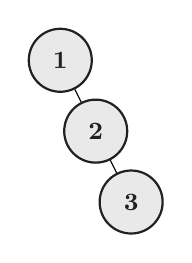
\begin{tikzpicture}[scale=0.6]
                \node[blacknode] {1}
                    child[missing] {}
                    child {node[blacknode] {2}
                        child[missing] {}
                        child {node[blacknode] {3}}
                    };
            \end{tikzpicture}
        \end{center}
        
        \column{0.33\textwidth}
        \pause
        \begin{center}
            \textbf{After 4}\\[0.3cm]
            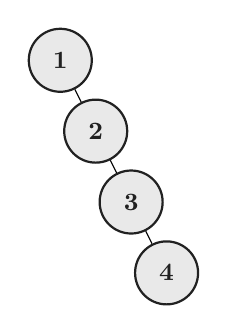
\begin{tikzpicture}[scale=0.6]
                \node[blacknode] {1}
                    child[missing] {}
                    child {node[blacknode] {2}
                        child[missing] {}
                        child {node[blacknode] {3}
                            child[missing] {}
                            child {node[blacknode] {4}}
                        }
                    };
            \end{tikzpicture}
        \end{center}
        
        \column{0.33\textwidth}
        \pause
        \begin{center}
            \textbf{After 5}\\[0.3cm]
            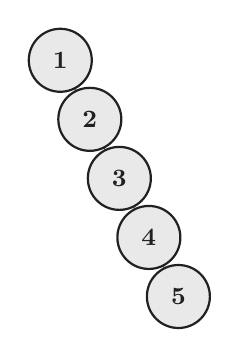
\begin{tikzpicture}[scale=0.5]
                \node[blacknode] {1}
                    child[missing] {}
                    child {node[blacknode] {2}
                        child[missing] {}
                        child {node[blacknode] {3}
                            child[missing] {}
                            child {node[blacknode] {4}
                                child[missing] {}
                                child {node[blacknode] {5}}
                            }
                        }
                    };
            \end{tikzpicture}
        \end{center}
    \end{columns}
    
    \vspace{0.5cm}
    \pause
    \begin{center}
        \Large\textbf{Our tree became a... \textcolor{rbred}{LINKED LIST!}}
    \end{center}
\end{frame}

% Performance degradation
\begin{frame}{From Sports Car to Bicycle}
    \begin{columns}
        \column{0.5\textwidth}
        \begin{block}{Before (Balanced)}
            \begin{itemize}
                \item Search: $O(\log n)$
                \item Insert: $O(\log n)$
                \item Delete: $O(\log n)$
            \end{itemize}
        \end{block}
        
        \begin{center}
            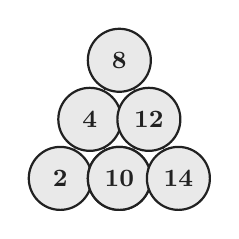
\begin{tikzpicture}[scale=0.5]
                \node[blacknode] {8}
                    child {node[blacknode] {4}
                        child {node[blacknode] {2}}
                        child {node[blacknode] {6}}
                    }
                    child {node[blacknode] {12}
                        child {node[blacknode] {10}}
                        child {node[blacknode] {14}}
                    };
            \end{tikzpicture}
        \end{center}
        
        \column{0.5\textwidth}
        \begin{alertblock}{After (Degenerate)}
            \begin{itemize}
                \item Search: $O(n)$
                \item Insert: $O(n)$
                \item Delete: $O(n)$
            \end{itemize}
        \end{alertblock}
        
        \begin{center}
            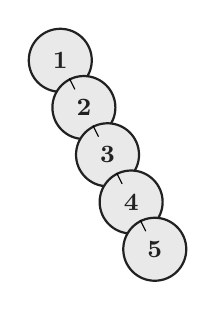
\begin{tikzpicture}[scale=0.4]
                \node[blacknode] {1}
                    child[missing] {}
                    child {node[blacknode] {2}
                        child[missing] {}
                        child {node[blacknode] {3}
                            child[missing] {}
                            child {node[blacknode] {4}
                                child[missing] {}
                                child {node[blacknode] {5}}
                            }
                        }
                    };
            \end{tikzpicture}
        \end{center}
    \end{columns}
    
    \vspace{0.5cm}
    \pause
    \begin{center}
        \Large\textcolor{rbred}{\faIcon{exclamation-triangle} Not Great!}
    \end{center}
\end{frame}

% The solution - balanced trees
\begin{frame}{We Need Almost Balanced Trees}
    \begin{center}
        \Large We want to keep $O(\log n)$ operations \textbf{even in the worst case!}
    \end{center}
    
    \pause
    
    \vspace{0.5cm}
    
    \begin{block}{Popular Solutions}
        \begin{itemize}
            \item<2-> AVL Trees
            \item<3-> \textbf{Red-Black Trees} \faIcon{star}
            \item<4-> B-Trees
            \item<5-> Splay Trees
        \end{itemize}
    \end{block}
    
    \pause[6]
    
    \begin{center}
        \Large\textbf{Red-Black Trees are used EVERYWHERE!}
    \end{center}
\end{frame}

% Red-Black Tree introduction with joke
\begin{frame}{Enter: Red-Black Trees}
    \begin{columns}
        \column{0.6\textwidth}
        \begin{itemize}
            \item<1-> Around since the 1970s
            \item<2-> Used in Linux kernels
            \item<3-> Java's TreeMap and TreeSet
            \item<4-> Databases and file systems
        \end{itemize}
        
        \pause[5]
        
        \begin{alertblock}{Fun Fact}
            \small Even the original inventor \textbf{didn't mention} Red-Black Trees in his main DSA book!\\
            He introduced \textit{Left-Leaning Red-Black Trees} instead. \faIcon{laugh}
        \end{alertblock}
        
        \column{0.4\textwidth}
        \only<6->{
            \begin{center}
                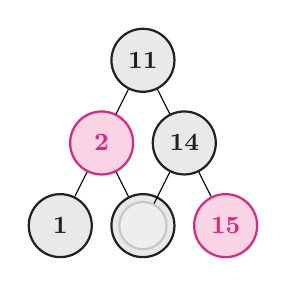
\begin{tikzpicture}[scale=0.7]
                    \node[blacknode] {11}
                        child {node[rednode] {2}
                            child {node[blacknode] {1}}
                            child {node[blacknode] {7}}
                        }
                        child {node[blacknode] {14}
                            child {node[nilnode] {}}
                            child {node[rednode] {15}}
                        };
                \end{tikzpicture}
            \end{center}
        }
    \end{columns}
    
    \vspace{0.3cm}
    \pause[7]
    \begin{center}
        \Large\textbf{Let's get started, shall we?}
    \end{center}
\end{frame}

% Fundamental properties introduction
\begin{frame}{Everything Has Unique Properties}
    \begin{center}
        \Large Fundamental properties are better than mathematical definitions!
    \end{center}
    
    \pause
    
    \vspace{0.5cm}
    
    \begin{columns}
        \column{0.5\textwidth}
        \begin{block}{Why Properties?}
            \begin{itemize}
                \item<2-> Easier to understand
                \item<3-> Audience feels good
                \item<4-> Been around for ages!
            \end{itemize}
        \end{block}
        
        \column{0.5\textwidth}
        \only<5->{
            \begin{center}
                \textbf{Red-Black Trees have 5 properties}\\[0.5cm]
                Let's see them \textcolor{rbred}{one by one}...
            \end{center}
        }
    \end{columns}
\end{frame}

% The Five Properties
\begin{frame}{The Five Properties}
    \begin{enumerate}
        \item<1-> Every node is either \textcolor{rbred}{Red} or \textcolor{rbblack}{Black}
        \item<2-> The \textbf{root} is always \textcolor{rbblack}{Black}
        \item<3-> All \textbf{leaves} (NIL) are \textcolor{rbblack}{Black}
        \item<4-> No two \textcolor{rbred}{Red} nodes can be adjacent
        \item<5-> Equal \textcolor{rbblack}{black height} on all paths
    \end{enumerate}
    
    \only<6->{
        \begin{center}
            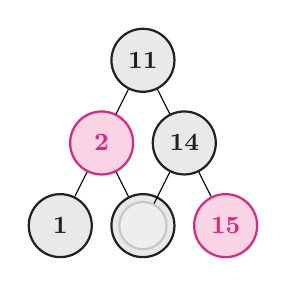
\begin{tikzpicture}[scale=0.7]
                \node[blacknode] {11}
                    child {node[rednode] {2}
                        child {node[blacknode] {1}}
                        child {node[blacknode] {7}}
                    }
                    child {node[blacknode] {14}
                        child {node[nilnode] {}}
                        child {node[rednode] {15}}
                    };
            \end{tikzpicture}
        \end{center}
    }
\end{frame}

% Black height explanation
\begin{frame}{Black Height: The Core Property}
    \begin{definition}
        The \textbf{black-height} of a node is the number of black nodes on any path from that node to a leaf (not counting the node itself).
    \end{definition}
    
    \pause
    
    \begin{center}
        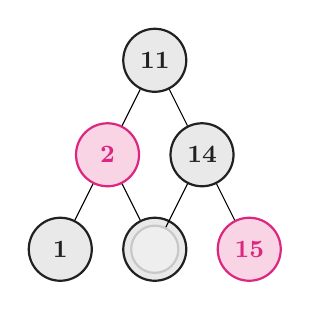
\begin{tikzpicture}[scale=0.8]
            \node[blacknode] (root) {11}
                child {node[rednode] {2}
                    child {node[blacknode] {1}}
                    child {node[blacknode] {7}}
                }
                child {node[blacknode] {14}
                    child {node[nilnode] {}}
                    child {node[rednode] {15}}
                };
        \end{tikzpicture}
    \end{center}
    
    \pause
    
    \begin{alertblock}{Why This Matters}
        This property helps us understand the \textbf{balance} of the tree!
    \end{alertblock}
\end{frame}

% Height bound (light touch)
\begin{frame}{The Amazing Height Bound}
    \begin{center}
        \Large Because of black height, we can prove:
    \end{center}
    
    \pause
    
    \begin{theorem}
        A Red-Black Tree with $n$ nodes has height $h \leq 2 \log_2(n+1)$
    \end{theorem}
    
    \pause
    
    \begin{columns}
        \column{0.5\textwidth}
        \begin{block}{What This Means}
            \begin{itemize}
                \item Even worst case is logarithmic!
                \item Never more than twice as tall as perfect tree
                \item $O(\log n)$ performance guaranteed
            \end{itemize}
        \end{block}
        
        \column{0.5\textwidth}
        \pause
        \begin{center}
            \textbf{Perfect Tree:} height = $\log_2(n+1)$\\[0.3cm]
            \textbf{RBT Tree:} height $\leq 2 \times \log_2(n+1)$\\[0.3cm]
            \Large\textcolor{green}{\faIcon{check} Still Awesome!}
        \end{center}
    \end{columns}
    
    \pause
    \begin{center}
        \small\textit{*(I skipped the detailed proof - nobody wants to sit through that!)*}
    \end{center}
\end{frame}

% Transition to operations
\begin{frame}{Wait, We're Not Done Yet!}
    \begin{center}
        \Large We haven't talked about \textbf{insertion} or \textbf{deletion} yet!
    \end{center}
    
    \pause
    
    \vspace{1cm}
    
    \begin{center}
        \Huge\textcolor{rbred}{\faIcon{exclamation-triangle}}\\[0.5cm]
        \Large\textbf{Warning: Shit's about to get real}\\[0.3cm]
        \large\textit{(Also tough)}
    \end{center}
    
    \pause
    
    \vspace{1cm}
    
    \begin{center}
        \Large\textbf{How do we insert something?}\\[0.5cm]
        \pause
        \large\textit{*(I know everybody knows...)*} \faIcon{smile}
    \end{center}
\end{frame}

% Insertion process
\begin{frame}{Insertion: The Process}
    \begin{enumerate}
        \item<1-> Insert like normal BST
        \item<2-> Color new node \textcolor{rbred}{RED}
        \item<3-> Fix any violations
    \end{enumerate}
    
    \only<4->{
        \begin{center}
            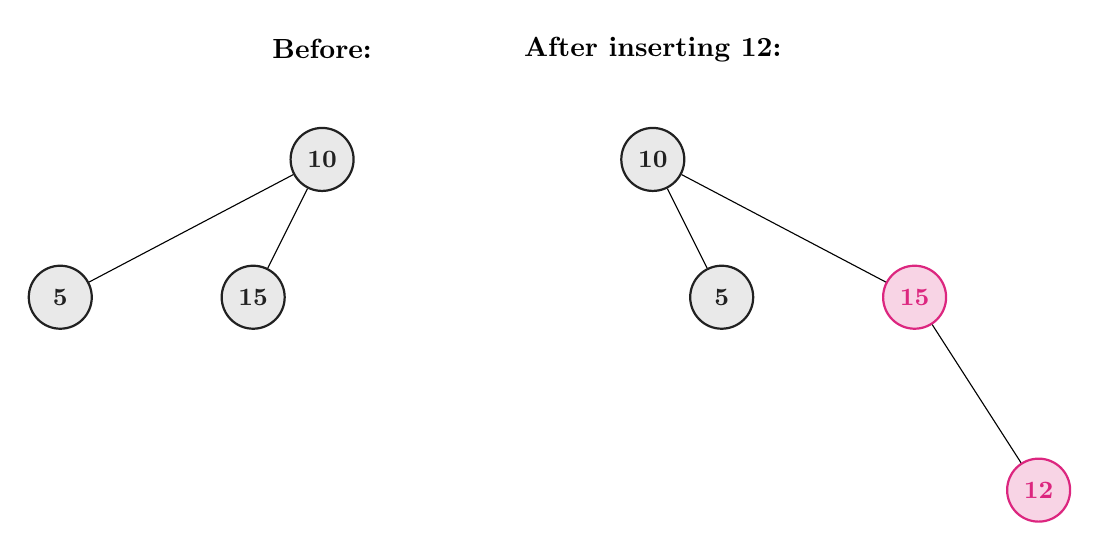
\begin{tikzpicture}[scale=0.7]
                % Before
                \node at (-3, 2) {\textbf{Before:}};
                \node[blacknode] at (-3, 0) {10}
                    child {node[blacknode] at (-4, -1) {5}}
                    child {node[blacknode] at (-2, -1) {15}};
                
                % After
                \node at (3, 2) {\textbf{After inserting 12:}};
                \node[blacknode] at (3, 0) {10}
                    child {node[blacknode] at (2, -1) {5}}
                    child {node[rednode] at (4, -1) {15}
                        child {node[rednode] at (3, -2) {12}}
                        child[missing] {}
                    };
            \end{tikzpicture}
        \end{center}
    }
    
    \only<5->{
        \begin{alertblock}{Problem!}
            We have two red nodes adjacent! Property 4 violated!
        \end{alertblock}
    }
\end{frame}

% Fixing violations
\begin{frame}{Fixing Violations}
    \begin{columns}
        \column{0.5\textwidth}
        \begin{block}{Uncle is RED}
            \begin{itemize}
                \item Easy case!
                \item Just recolor
                \item Flip parent, uncle, grandparent
            \end{itemize}
        \end{block}
        
        \pause
        
        \column{0.5\textwidth}
        \begin{alertblock}{Uncle is BLACK}
            \begin{itemize}
                \item Hard case!
                \item Need rotations
                \item Left rotate, right rotate
                \item Sometimes both!
            \end{itemize}
        \end{alertblock}
    \end{columns}
    
    \pause
    
    \vspace{0.5cm}
    
    \begin{center}
        \Large\textcolor{rbred}{This is where it gets tricky!}\\[0.3cm]
        \large But it keeps the tree balanced!
    \end{center}
\end{frame}

% Deletion (brief)
\begin{frame}{Deletion: Even More Fun!}
    \begin{center}
        \Large\textbf{Deletion is even more... interesting!} \faIcon{smile}
    \end{center}
    
    \pause
    
    \begin{columns}
        \column{0.5\textwidth}
        \begin{block}{If deleting RED node}
            \begin{itemize}
                \item No problem!
                \item Just remove it
                \item Properties still hold
            \end{itemize}
        \end{block}
        
        \column{0.5\textwidth}
        \pause
        \begin{alertblock}{If deleting BLACK node}
            \begin{itemize}
                \item Oh boy...
                \item Black height changes!
                \item Need "double black" fix
                \item Complex cases
            \end{itemize}
        \end{alertblock}
    \end{columns}
    
    \pause
    
    \vspace{0.5cm}
    
    \begin{center}
        \textbf{The key:} Maintain black height at all costs!\\[0.3cm]
        \large\textit{*(We'll skip the gory details - you get the idea!)*}
    \end{center}
\end{frame}

% Real-world applications
\begin{frame}{Where Are Red-Black Trees Used?}
    \begin{center}
        \Large\textbf{Everywhere!}
    \end{center}
    
    \pause
    
    \begin{columns}
        \column{0.5\textwidth}
        \begin{itemize}
            \item<2-> \faIcon{linux} \textbf{Linux Kernel}\\
                \small Process scheduling
            \item<3-> \faIcon{java} \textbf{Java}\\
                \small TreeMap, TreeSet
            \item<4-> \faIcon{database} \textbf{Databases}\\
                \small Indexing structures
            \item<5-> \faIcon{folder} \textbf{File Systems}\\
                \small Directory organization
        \end{itemize}
        
        \column{0.5\textwidth}
        \only<6->{
            \begin{center}
                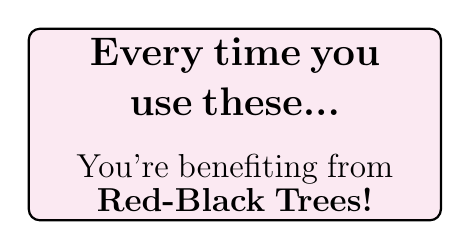
\begin{tikzpicture}
                    \node[draw, thick, rounded corners, fill=rbred!10, text width=5cm, align=center, minimum height=2cm] {
                        \Large\textbf{Every time you use these...}\\[0.3cm]
                        \large You're benefiting from\\
                        \textbf{Red-Black Trees!}
                    };
                \end{tikzpicture}
            \end{center}
        }
    \end{columns}
\end{frame}

% Conclusion
\begin{frame}{So There You Have It!}
    \begin{center}
        \Large\textbf{Red-Black Trees in a Nutshell}
    \end{center}
    
    \pause
    
    \begin{columns}
        \column{0.6\textwidth}
        \begin{itemize}
            \item<2-> Complex but incredibly powerful
            \item<3-> Tricky to implement
            \item<4-> Guaranteed $O(\log n)$ performance
            \item<5-> Used everywhere in computing
        \end{itemize}
        
        \column{0.4\textwidth}
        \only<6->{
            \begin{center}
                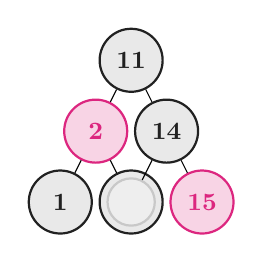
\begin{tikzpicture}[scale=0.6]
                    \node[blacknode] {11}
                        child {node[rednode] {2}
                            child {node[blacknode] {1}}
                            child {node[blacknode] {7}}
                        }
                        child {node[blacknode] {14}
                            child {node[nilnode] {}}
                            child {node[rednode] {15}}
                        };
                \end{tikzpicture}
            \end{center}
        }
    \end{columns}
    
    \pause[7]
    
    \vspace{0.5cm}
    
    \begin{center}
        \begin{alertblock}{Remember}
            The next time you're struggling with RBT implementation...\\[0.3cm]
            \large Even the \textbf{inventor} moved on to Left-Leaning Red-Black Trees! \faIcon{laugh}
        \end{alertblock}
    \end{center}
    
    \pause
    
    \begin{center}
        \Large\textbf{Thanks for listening!}\\[0.3cm]
        \large May your trees always stay balanced! \faIcon{tree}
    \end{center}
\end{frame}

% Questions slide
\begin{frame}
    \begin{center}
        \Huge\textbf{Any Questions?}\\[1cm]
        \Large\faIcon{comments}
    \end{center}
\end{frame}

\end{document}
